\section{Problem Statement}
\label{sec:problem}
As mentioned before, our focus in this work is to
generate the most prominent aspects of a given product type
from textual reviews.
More specifically, the problem is defined as:
given all the text reviews about
one type of product or service, extract $K$ words (or phrases),
each of which represents a prominent and distinct review aspect.
For instance, if the given product type is \textit{hotel}, 
we expect a successful extraction framework to extract 
$K=5$ aspect terms as follows: 
\textit{room, location, staff, breakfast, pool}.
Here $K$ is a constant parameter for the problem. 
The set of reviews and the number of aspects are inputs.


\paragraph{Definition 1}
We term the problem as \textit{Prominent Aspect Extraction},
which aims to find 
%Following the above discussions, next we formally describe our
%problem which we term as . 
an optimal set of $K$ aspects $[a_1, a_2, ..., a_K]$, such that:
\begin{itemize}
	\item  the $K$ aspects cover as much aspect space $C$ as possible,
	i.e. maximizing $\bigcup_{k=1}^K c(a_k)$;
	\item the semantic overlaps between those aspects are minimum, 
	i.e. minimizing $\sum_{i=1}^{K}\sum_{j=1}^{K}o(a_i, a_j)$,
\end{itemize}
where $c(a_k)$ denotes the semantic coverage of the aspect $a_k$,
and $o(a_i, a_j)$ represents the semantic overlaps between 
$a_i$ and $a_j$.

The challenges in a good choice of $a_1\sim a_K$ are properly
formulating the \textit{semantic coverage} and \textit{semantic overlaps}.
To formulate the aspect space with minimum noise, 
ExtRA builds an aspect graph specialized for the given type of product.
Then, we propose a novel strategy which segments the space into reasonable aspect clusters in order to model the semantic coverage of
aspects more accurate, since the potential prominent aspects can benefit from other members within the same cluster.
Finally, we generate the prominent aspects from aspect clusters
by utilizing the internal structure of each aspect cluster.

Note that in this definition we don't use cross-domain information, 
that is, for one product type we only use the reviews of that domain.
Thus, our model can extract aspects from any domain as long as the reviews for that domain is available.

\section{Methodology}
\figref{fig:flow} depicts the architecture of ExtRA.
The collection of customer reviews and the
number of prominent aspects to extract are inputs.
ExtRA extracts the aspect candidates from text reviews and
aggregates them into aspect synsets to construct the aspect space.
Next, it builds an aspect graph utilizing the Probase to narrow the aspect space, then segments the space into aspect clusters 
utilizing strategies of relation weighting and grouping,
and finally generates the top \emph{K} prominent aspects from aspect clusters.
ExtRA makes use of external knowledge such as Probase, WordNet and word embeddings (i.e. Glove~\cite{pennington2014glove}).

\begin{figure}[th!]
	\centering
	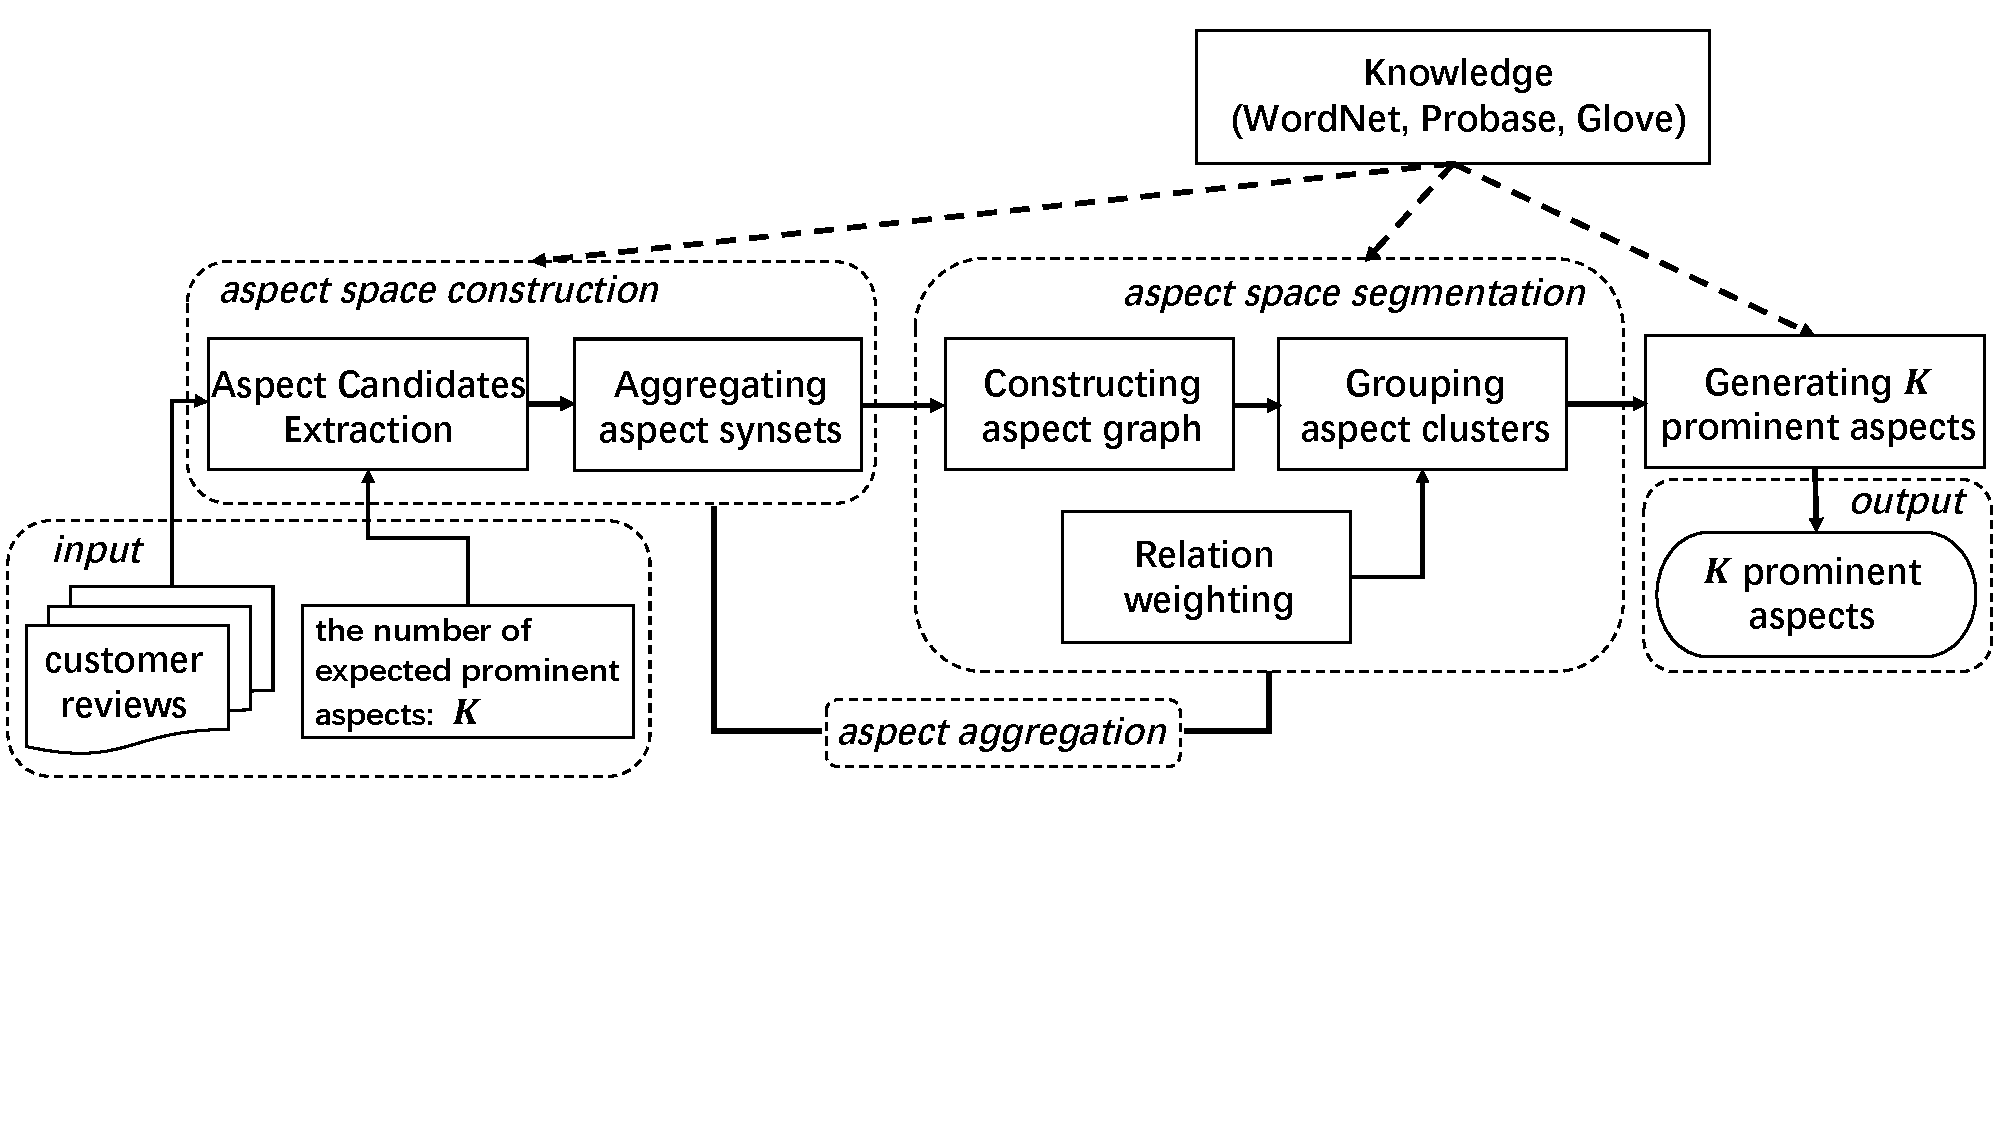
\includegraphics[width=0.95\columnwidth]{figures/nflow}
	\caption{The architecture of ExtRA}
	\label{fig:flow}
\end{figure}

\subsection{Aspect Candidates Extraction}
\label{sec:candidate}
Following the observation of Liu~\cite{hu2004mining,liu2015automated}, 
we assume that aspect terms are nouns and noun phrases.  
First, we design a set of effective syntactic rules, which can be applied across domains, to collect the aspect candidates from review texts.
We mainly use the adjectival modifier dependency relation (\emph{amod})
and the nominal subject relation (\emph{nsubj})
to extract the aspect-opinion pairs $\left\langle N, A \right\rangle$.
In addition, we leverage the conjunction relation (\emph{conj}) between 
adjectives to complement the extracted pairs. 
Formally, the extraction rules can be specified as follows:
\begin{description}
	\item [Rule 1.] If $amod(N, A)$, then extract $\left\langle N, A \right\rangle$.
	\item [Rule 2.]If $nsubj(A, N)$, then extract $\left\langle N, A \right\rangle$.
	\item [Rule 3.]If $\left\langle N, A_i \right\rangle$ and $conj(A_i, A_j)$, then extract $\left\langle N, A_j \right\rangle$.
\end{description}
In this case, $N$ indicates a noun, 
%$N_{-1}$ and $N_{+1}$ also denotes the noun word, 
%and the subscript represents displacement to $N$.
and $A$ (e.g. $A_i$, $A_j$) is an adjective. 
The dependencies (e.g. $amod(N, A)$) are expressed as $rel(head, dependent)$, where \textit{rel} is the dependency relation which holds
between \textit{head} and \textit{dependent}.
Note that many aspects are expressed by phrases,
thus, we introduce \emph{noun compound} relation 
(abbreviated \emph{comp}) to
extend phrases as aspect candidates.
The phrase extension rules for the extracted aspect-opinion pair $\left\langle N, A \right\rangle$ are as follows:
\begin{description}
	\item [Rule E1.] If $\left\langle N, A \right\rangle$ and $comp(N_{-1}, N)$, then use $\left\langle N_{-1}\_N, A \right\rangle$ to replace $\left\langle N, A \right\rangle$;
	\item [Rule E2.] If $\left\langle N, A \right\rangle$ and $comp(N, N_{+1})$, then use $\left\langle N\_N_{+1}, A \right\rangle$ to replace $\left\langle N, A \right\rangle$;
	\item [Rule E3.] If $\left\langle N, A \right\rangle$ and $amod(V_{-1}, N)$, then use $\left\langle V_{-1}\_N, A \right\rangle$ to replace $\left\langle N, A \right\rangle$,
\end{description}
where $N_{-1}$ and $N_{+1}$ denotes the noun word, $V_{-1}$ is the gerund, 
and the subscript represents the displacement to $N$ in the sentence.
Note that in order to obtain more accurate aspect candidates,
we aim to extract the sentiment aspect-opinion pairs. 
We constrain that the opinion word $A$ of each pair $\langle$N, A$\rangle$ is in the sentiment opinion lexicon proposed by Liu\cite{hu2004mining}.

\begin{table}[th!]
	\small
	\begin{center}
		\caption{The extraction of opinion-aspect pairs from review sentences.} 
		\label{table:extraction}
		\begin{tabular}{l P{2cm} P{3.2cm}}
			\toprule
			%		\hline
			\textbf{Review sentences} & \textbf{Rules} & \textbf{Opinion-aspect pairs} \\
			\cmidrule(r){1-1}\cmidrule(lr){2-2}\cmidrule(l){3-3}
			\raisebox{-0.5\totalheight}{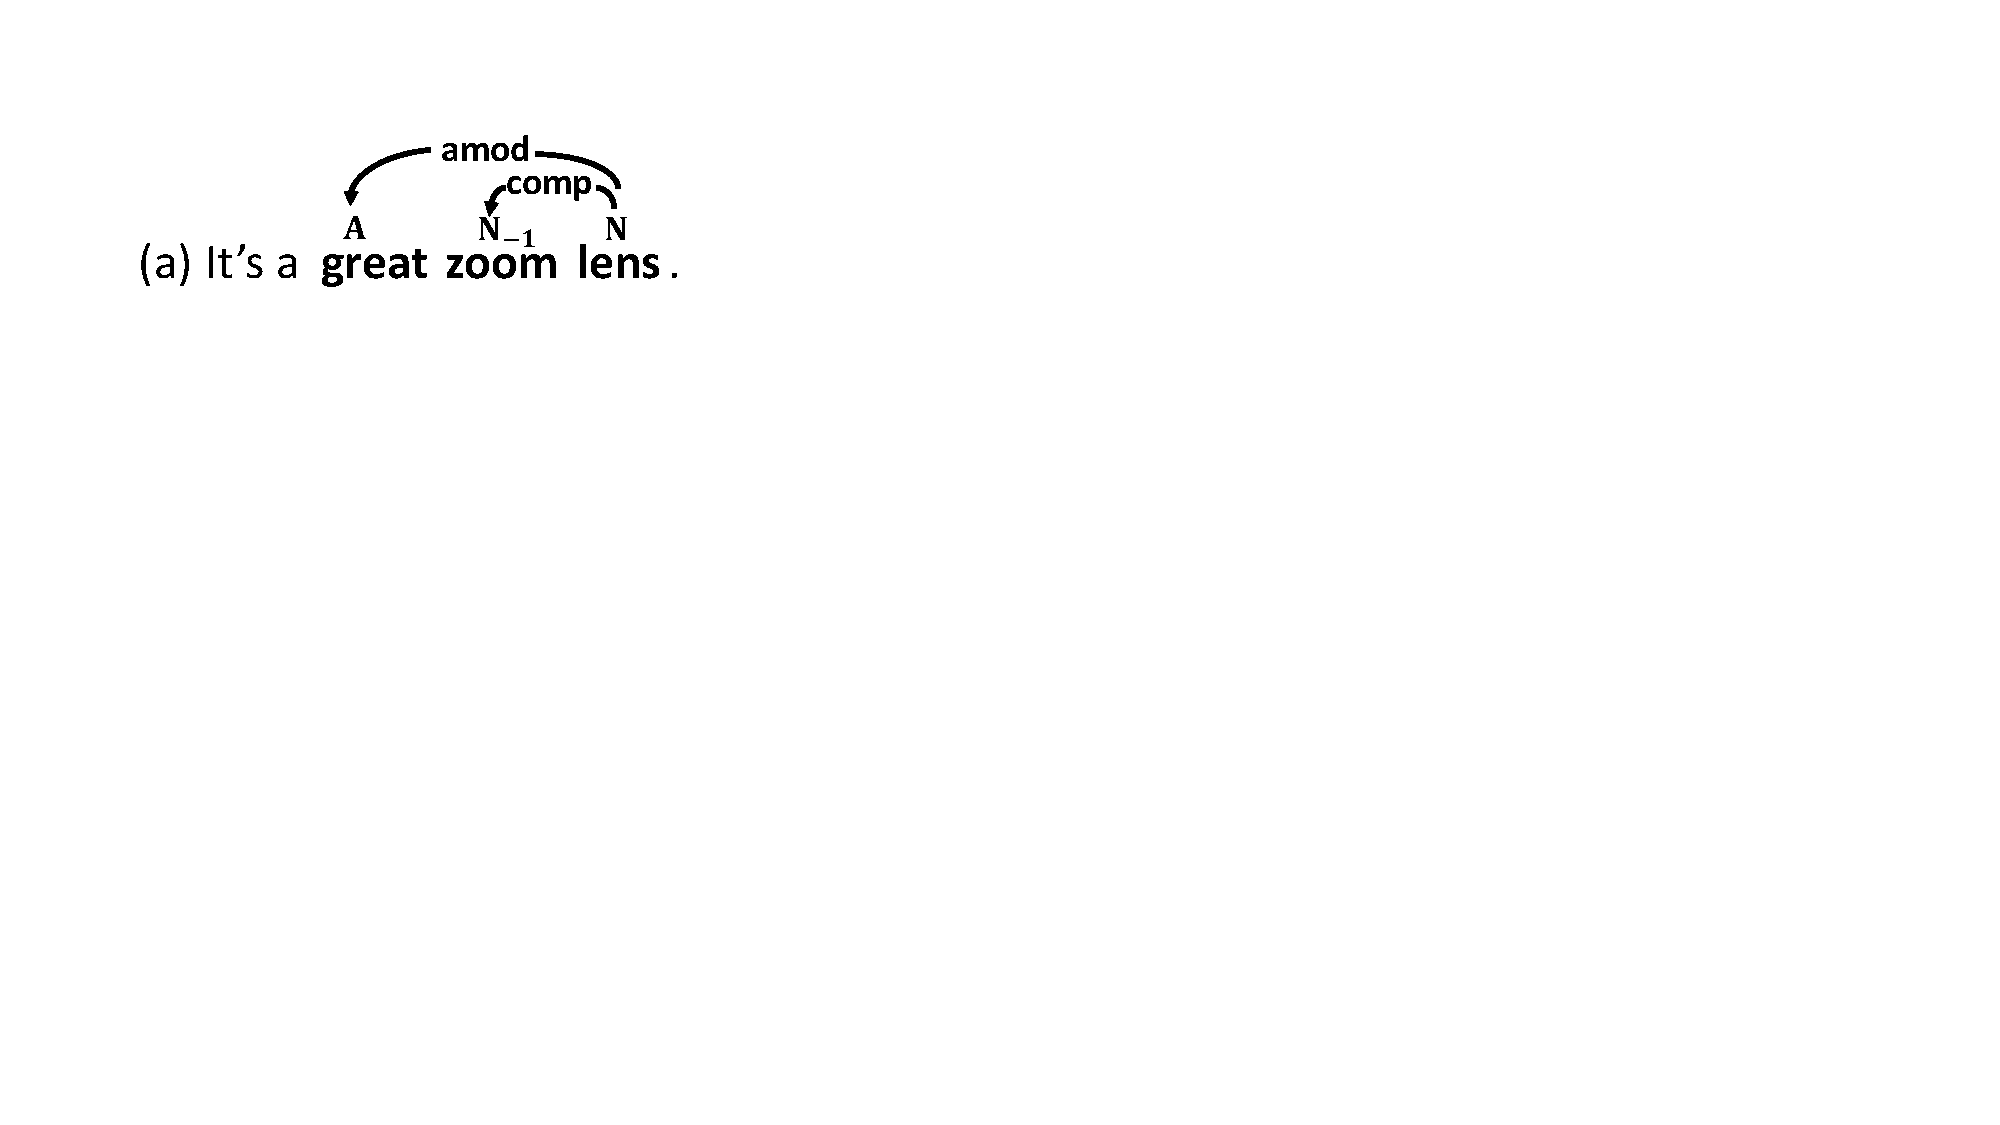
\includegraphics[width=0.4\textwidth]{figures/extraction_a}}  & 
			\raisebox{-0.25\totalheight}{
				\begin{tabular}{c}
					\textbf {Rule 1.} \\ 
					\textbf {Rule E1.} \\
			\end{tabular}}  & 
			\raisebox{-0.25\totalheight}{
				\begin{tabular}{c}
					\st{$\langle$great, lens$\rangle$} \\ 
					$\langle$great, zoom lens$\rangle$ \\
			\end{tabular}} \\\hline
			\raisebox{-\totalheight}{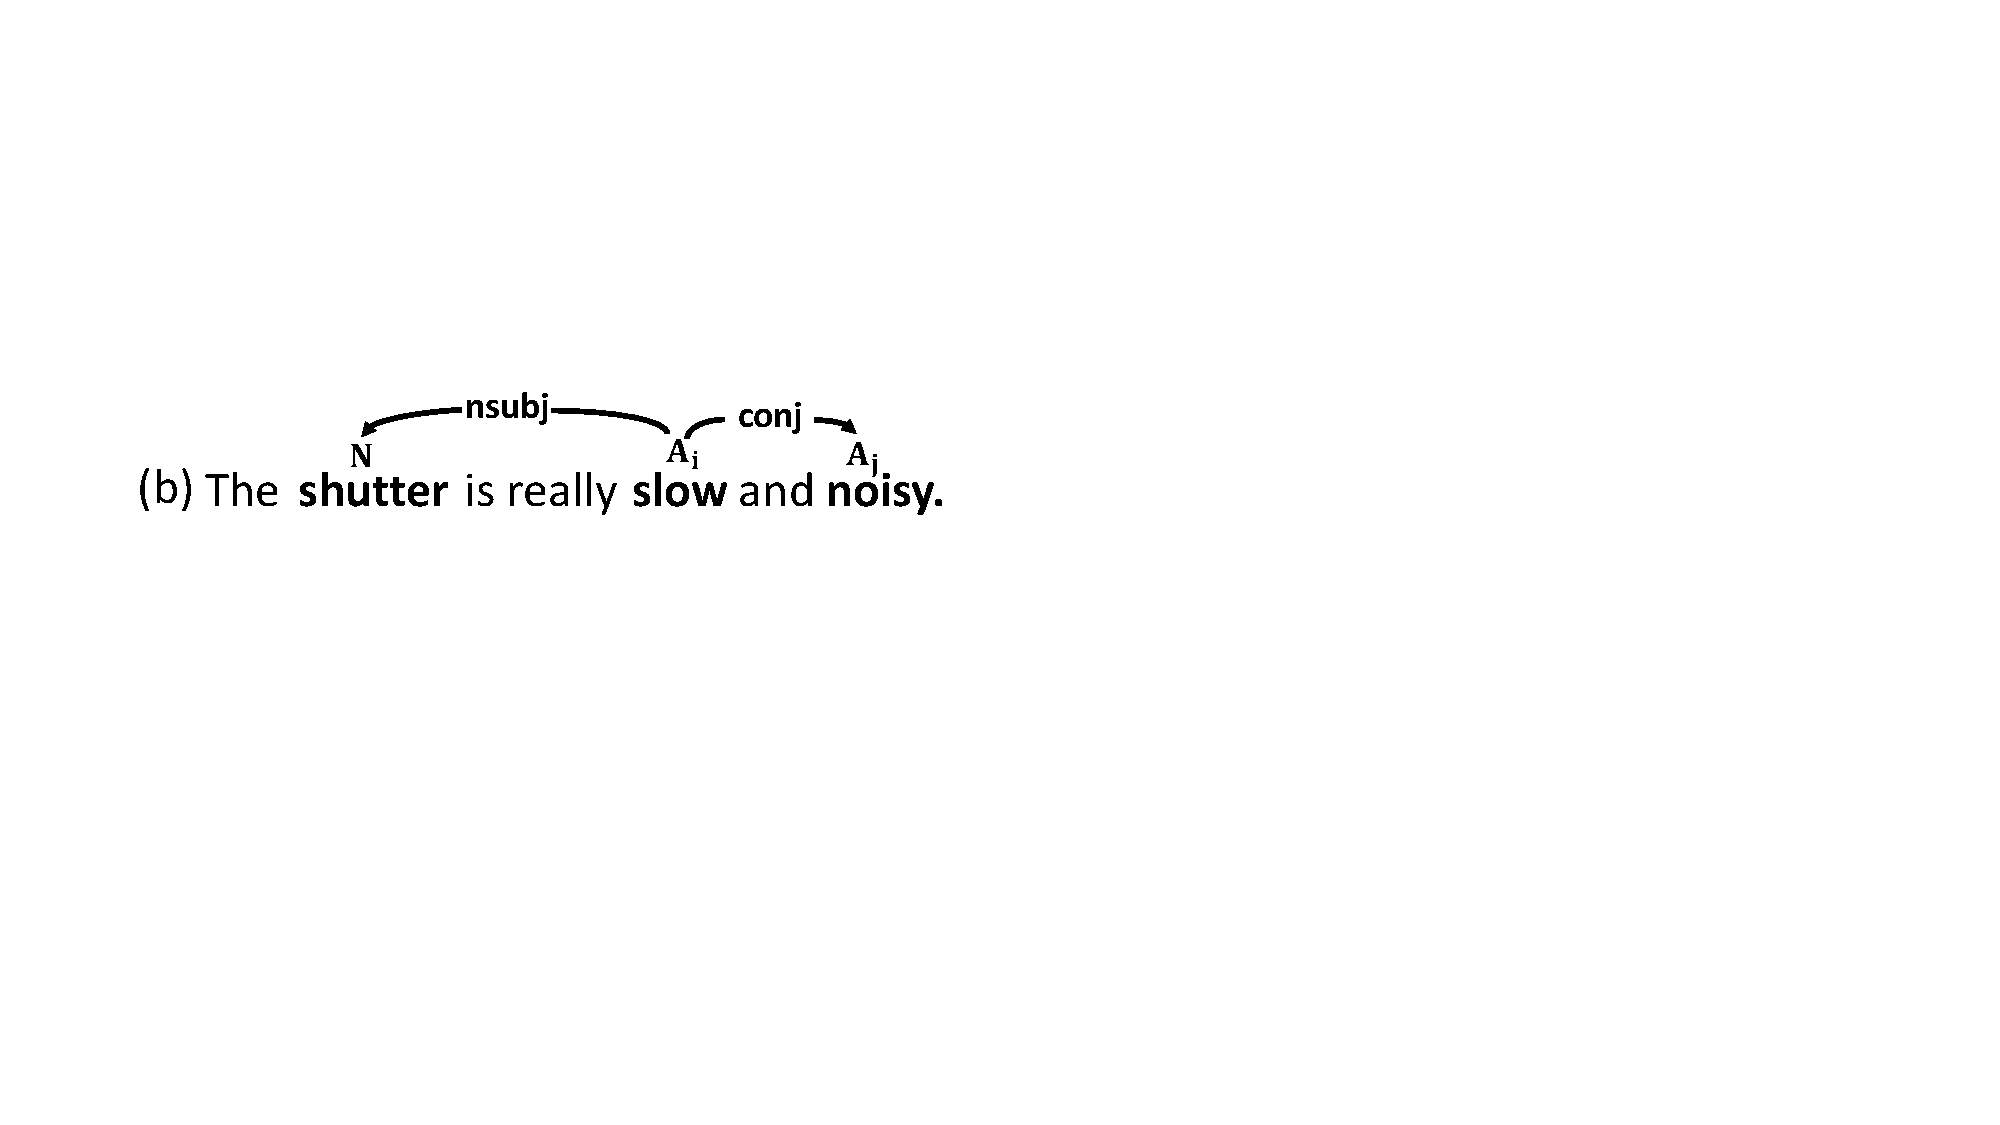
\includegraphics[width=0.4\textwidth]{figures/extraction_b}} & 
			\raisebox{-0.75\totalheight}{
				\begin{tabular}{c}
					\textbf {Rule 2.} \\ 
					\textbf {Rule 3.} \\
				\end{tabular}
			}  &
			\raisebox{-0.75\totalheight}{
				\begin{tabular}{c}
					$\langle$slow, shutter$\rangle$ \\ 
					$\langle$noisy, shutter$\rangle$ \\
			\end{tabular}} \\\hline
			\raisebox{-\totalheight}{
				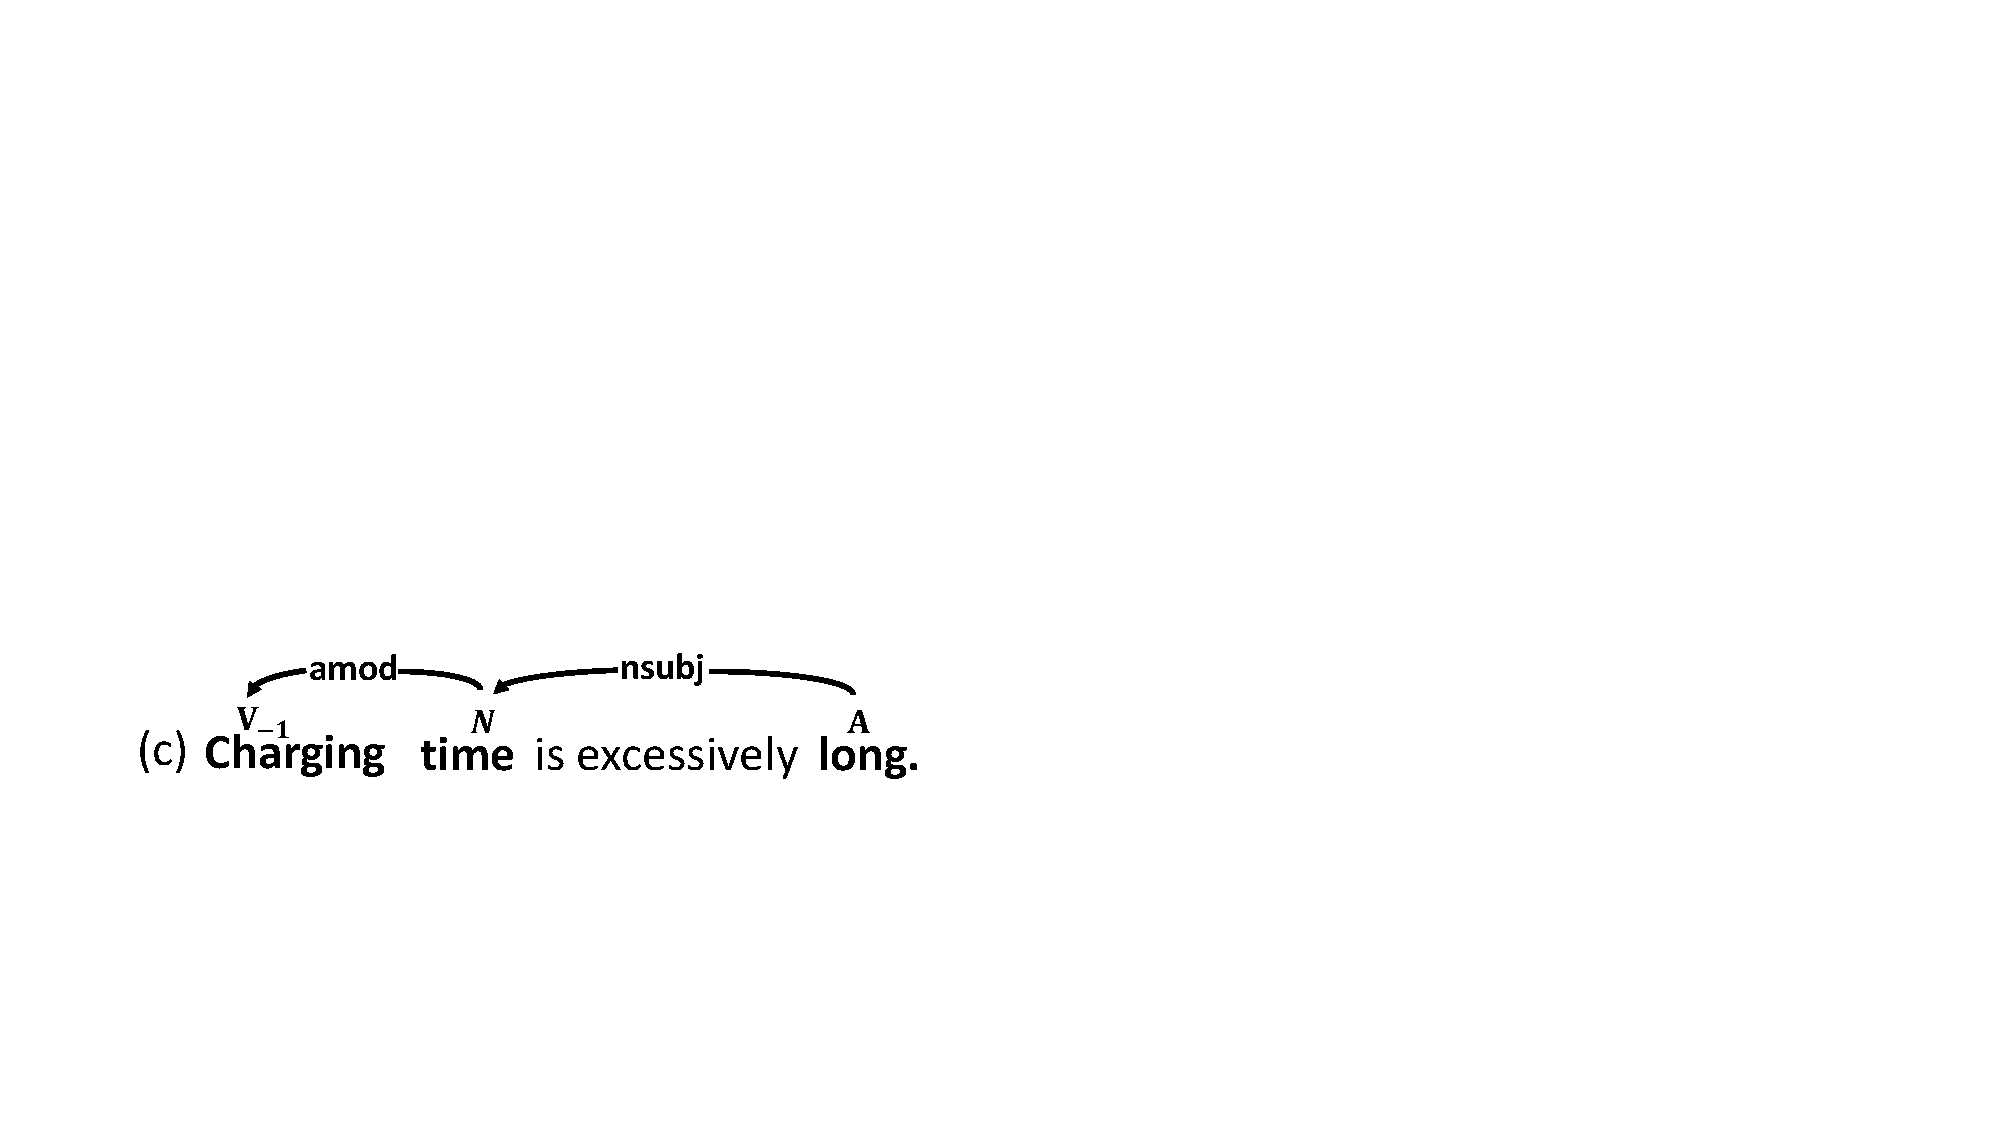
\includegraphics[width=0.4\textwidth]{figures/extraction_c}}   &
			\raisebox{-0.75\totalheight}{
				\begin{tabular}{c}
					\textbf {Rule 2.} \\ 
					\textbf {Rule E3.} \\
				\end{tabular}
			}  & 
			\raisebox{-0.75\totalheight}{
				\begin{tabular}{c}
					\st{$\langle$long, time$\rangle$} \\ 
					$\langle$long, changing time$\rangle$ \\
			\end{tabular}} \\\hline
		\end{tabular}
	\end{center}
\end{table}









\tabref{table:extraction} demonstrates the extraction process using
some example sentences with syntactic features. 
For example, in sentence (a), we first extract the pair $\langle$\emph{great}, \emph{lens}$\rangle$ by applying \emph{Rule 1}, then we 
replace that pair with $\langle$\emph{great}, \emph{zoom\_lens}$\rangle$
by applying \emph{Rule E1}. 
Similarly, the extraction rules match
$\langle$\emph{slow}, \emph{shutter}$\rangle$, $\langle$\emph{noisy}, \emph{shutter}$\rangle$
in sentence (b) and $\langle$\emph{long}, \emph{charging\_time}$\rangle$ in sentence (c) as potential aspect-opinion pairs.

After extracting such aspect-opinion pairs from the text reviews, we use $freq(\left\langle N, A\right\rangle)$ to represent the number
of occurrences of $\left\langle N, A \right\rangle$.
The frequency of the aspect $N$ 
(i.e. $freq(N)$) is computed as: 
\begin{equation}
	freq(N) = \sum\limits_{\left\langle N,A\right\rangle \in P}{freq(\left\langle N, A\right\rangle )},
\end{equation}
where $P$ is the set of aspect-opinion pairs extracted
from the corpus.
We sort the extracted aspects by frequency,
and consider the top 1000 of them
as aspect candidates, assuming that
the most prominent aspects are subsumed by those candidates terms. 


\subsection{Aspect Aggregation}
We collect a bunch of aspect candidates from the previous extraction stage. 
The \textit{prominent aspects} are supposed
to be important and popular but sometimes coarse-grained, which 
means they may semantically cover or overlap with a set of other aspect 
candidates.
The simplest method is to extract the most frequent $K$ aspect candidates as the $K$ expected prominent aspects
since the frequency is a natural measure of popularity (or importance).
However, the expression of the prominent aspect 
can be highly versatile. 
For example, \textit{os}, 
\textit{operating system}
and \textit{Windows XP}
describe the same prominent aspect of Laptop: 
\textit{operating system}.
Therefore, it is reasonable
to aggregate the aspects which are about the same 
prominent aspect together to enhance the popularity. 
We aggregate the aspect candidates 
into clusters following two principles:
\begin{itemize}
	\item  Aggregate the aspects with high semantic overlaps into \textit{aspect synsets}.
	%	such as \textit{os} and \textit{operating system};
	\item Group the \textit{aspect synsets} 
	with high semantic subsumption into \textit{aspect clusters}.
	%	 such as \textit{operating system} and \textit{Windows XP}. 
\end{itemize}

In this section, we first aggregate the aspect candidates into aspect synsets in \secref{sec:aspect_synsets}, 
ensuring that the candidates
which refer to the same aspect are attached with
each other.  
Then, we narrow the aspect space from the original set of  aspect candidates 
to the set of nodes (aspects) of the constructed aspect graph in
\secref{sec:clusters}. 
Finally, we utilize the proposed relation weighting scheme 
to segment the aspect space into clusters.


\subsubsection{Aspect synsets}
\label{sec:aspect_synsets}
We use WordNet and Glove to aggregate the aspect candidates with highly semantic overlaps into \textit{aspect synsets}.
\textit{Aspect synonyms} are the aspects that 
have similar meanings.  
\textit{Aspect synset} is a group of
aspect synonyms. 
The algorithm of aspect synsets generation is described in 
\algoref{alg:aspect_synonyms}.
\begin{algorithm}[!th]
	\small
	\KwIn{A list of aspects $N = [n_1, n_2, ..., n_M]$ sorted by frequency in descending order.}
	\KwOut{A list of aspect synsets $S=[s_1, s_2, ..., s_T]$ sorted by priority in descending order.}
	\BlankLine
	%	Initializing aspect synsets as $S=[s_1, s_2, ..., s_M]$, where $s_i=\{N_i\}$\;
	$S \leftarrow []$\;
	$toSkip \leftarrow \emptyset$\;
	\For{$i \leftarrow 1$ \KwTo $M$}{
		\If{$n_i \in toSkip $}{continue;}
		$t \leftarrow len(S)$\;
		$s_t \leftarrow \{n_i\}$\;
		$L_i \leftarrow lemmas(n_i)$\;
		\For{$j \leftarrow i+1$ \KwTo $M$}{
			\If{$n_j \in toSkip $}{continue;}
			$L_j \leftarrow lemmas(n_j)$\;
			\If{$n_i \in L_j$ {\bf and} $n_j \in L_i$ {\bf or} $sim(n_i, n_j) \ge thred$}{$s_t \leftarrow s_t \cup \{n_j\}$\; $toSkip \leftarrow toSkip \cup \{n_j\}$;}
			\For{$n \in L_j$}{
				\If{$n \in N$ {\bf and} $n_j \in lemmas(n)$ {\bf or} $sim(n, n_j) \ge thred$} {$s_t \leftarrow s_t \cup \{n\}$\; 
					$toSkip \leftarrow toSkip \cup \{n\}$;}
			}
		}
		Append $s_t$ to $S$\;
		$toSkip \leftarrow toSkip \cup \{n_i\}$\;
	}
	Sort $S$ by priority in descending order\;
	{\bf return} $S$\;
	\caption{Aspect Synsets Generation \label{alg:aspect_synonyms}}
\end{algorithm}

\paragraph{WordNet}
The WordNet organizes words with similar meanings
as \textit{synsets}.
A \textit{synset} represents a specific sense of a specific word.
Each synset contains one or more lemmas, 
vice versa,
one lemma can belong to one or more synsets.
Thus, it is intuitive to take the aspects
that belong to the same \textit{synset} as the aspect synonyms.
Such aspect synonyms are supposed to have 
the same meaning at least in one sense.
%The intuition of the aggregation using WordNet
%is to group the aspects belonging to the same WordNet \textit{synset} together.
%At first, each aspect (e.g. $N$) is treated as an \textit{aspect synset} (e.g. $s=\{N\}$).
We ensure that each aspect (i.e. $n$) is assigned to
only one \textit{aspect synset} using
\algoref{alg:aspect_synonyms}.
$lemmas(n)$ represents the set of all synonyms 
for $n$.
For example, word $n$ have $m$ senses which correspond to
one synset each in WordNet.
$l(s)$ is the set of synonyms of synset $s$.
Then, $lemmas(n)=\bigcup\limits_{i=1}^{m} l(s_i)$.
Note that 
the priority of each \textit{aspect synset} (e.g. $s$) is 
computed as: 
\begin{equation}
	\sum\limits_{n \in s}freq(n).
	\label{eq:priority}
\end{equation}
Such aggregation groups \textit{os} and \textit{operating system} together.

\paragraph{Glove}
While WordNet is powerful, the synsets information for phrases 
in WordNet is not as rich as words.
For example, we expect to group \textit{pool} and \textit{swimming pool} which are almost the same
meaning in semantics 
together, though they do not 
have the same sense in WordNet.
To ameliorate this limitation,
we introduce word embeddings
which are widely used for capturing the semantic similarity (i.e. semantic overlap)
between words and phrases.
We calculate the semantic overlap between the term $n_i$ and $n_j$ as $sim(n_i, n_j)$, which is the cosine similarity 
computed by Glove embeddings. 
If $n_i$ is a phrase composed by words $[w_1, ..., w_K]$,
then $E(n_i)$, the embedding of $n_i$, 
is calculated as: 
\begin{equation}
	E(n_i) = \sum\limits_{k=1}^{K}E(w_k). 
	\label{eq:embedding}
\end{equation}
We set the threshold $thred$ to be very high (i.e. $0.9$)
in order to group aspect synonyms in \algoref{alg:aspect_synonyms}.

%\subsubsection{Semantic Coverage}
\subsubsection{Aspect Clusters}
\label{sec:clusters}
In this section, we aggregate the aspect synsets
into aspect clusters.
Each aspect cluster implies a prominent aspect
for the given product or service.
We expect to 
capture the hierarchical structure between aspects
and to group those hypernym-hyponym aspects together.
For example, 
 \textit{Windows XP} is the hyponym aspect of
\textit{operating system}, which means \textit{Windows XP} is
a kind of \textit{operating system}.

\paragraph{Probase}
We leverage Probase~\cite{wu2012probase} to identity \textit{isA} relations
between aspects.
Probase is a data-driven semantic network that
consists of millions of fine-grained concepts
and their \textit{isA} relationships.
Thus, it is more suitable than WordNet on measuring
the semantic subsumptions between aspects.
For an \textit{isA} relationship $\left\langle u,v\right\rangle$ from Probase, 
the hypernym $u$ is called \textit{concept},
and the hyponym $v$ is called \textit{entity} or \textit{instance}.
Each relationship $\left\langle u,v\right\rangle$
is associated with the number of occurrences (i.e. $f(\left\langle u,v\right\rangle)$)
that $u$ occurred as the concept of $v$ in the corpus.
If $f(\left\langle u,v\right\rangle)$ is greater than 100,
we consider that there is an isA relationship between $u$
and $v$. In other words, $v$ is semantically covered 
by $u$ in the commonsense.

\begin{algorithm}[!th]
	\small
	\KwIn{The set of aspect candidates $N=\{n_1, n_2, ..., n_M\}$.}
	\KwOut{$G=(V, E)$.}
	\BlankLine
	$V \leftarrow \emptyset$\;
	$E \leftarrow \emptyset$\;
	\For{$i \leftarrow 1$ \KwTo $M$}{
		\For{$j \leftarrow i+1$ \KwTo $M$}{
			\If{$n_j \in topEntities(n_i)$ {\bf and} $n_i \in topConcepts(n_j)$}{
				$E \leftarrow E \cup \{\left\langle n_i, n_j \right\rangle\}$\;
			}
			\If{$n_i \in topEntities(n_j)$ {\bf and} $n_j \in topConcepts(n_i)$}{
				$E \leftarrow E \cup \{\left\langle n_j, n_i \right\rangle\}$\;
			}
		}
	}
	\For{$\left\langle u,v\right\rangle \in E$}{
		$V \leftarrow V \cup \{u\}$\;
		$V \leftarrow V \cup \{v\}$\;
	}
	{\bf return} G \;
	\caption{Aspect Graph Construction\label{alg:relations}}
\end{algorithm}

\paragraph{Aspect graph construction}
Given the extracted aspect candidates,
we first extract an aspect graph $G=(V, E)$ from Probase.
Each node $v\in V$ is an aspect candidate.
Each edge $e=\left\langle u,v\right\rangle$,
directed from the concept $u$ to the entity $e$,
represents an isA relationship from Probase.
To improve the quality of relationships in $G$,
we only reserve top frequent relationships
for both $u$ and $v$. The algorithm for the graph
construction is described in \algoref{alg:relations}.
 $topEntities(n)$ returns the top 20 frequent entities
 for the concept $n$, and $topConcepts(n)$ returns
 the top 20 frequent concepts for the entity $n$.

\paragraph{Relation weighting}
In order to measure the quality of each relationship 
$\left\langle u,v \right\rangle$ in $G$,
we propose a weighting scheme for 
$\left\langle u,v \right\rangle$.
According to Wu\cite{wu2012probase}, 
each relationship $\left\langle u,v \right\rangle$ 
is associated with 
two typicalities, $\mathcal{T}(u|v)$ and $\mathcal{T}(v|u)$,
which are useful for 
conceptualization and inference.
$\mathcal{T}(u|v)$ is the typicality of the concept $u$
given the instance $v$, and
$\mathcal{T}(v|u)$ is the typicality of the instance $v$ given 
the concept $u$.
In our scenario, they are computed as follows:
\begin{equation}
	\mathcal{T}(u|v) = \frac{f(\left\langle u,v \right\rangle)}{f(v)}
\end{equation}

\begin{equation}
\mathcal{T}(v|u) = \frac{f(\left\langle u,v \right\rangle)}{f(u)},
\end{equation}
where $f(u)$ (or $f(v)$) is the frequency of $u$ (or $v$)
acting as the concept (or instance) in Probase.
The weight of the edge $\left\langle u,v \right\rangle$
is computed as:
\begin{equation}
	w(\left\langle u,v \right\rangle) = \mathcal{T}(u|v)^{\frac{1}{2}} *\mathcal{T}(v|u)^{\frac{1}{2}}
	\label{eq:weighing}
\end{equation}
This scheme captures the intuition
that if $u$ associates more typically to $v$ or vice versa,
$\left\langle u,v \right\rangle$ is often weighted higher. 
%In prominent aspect extraction, 
%the semantic of hyponym aspect is usually covered by 
%that of the hypernym aspect.
\paragraph{Grouping}
\label{para:grouping}
If $\left\langle u,v\right\rangle \in E$ and
$\left\langle v,u\right\rangle \in E$, in another word,
$u$ is an instance of $v$ and vice versa, 
then we take $u$ and $v$ as aspect synonyms.
Thus, if $u \in s_u$ and $v \in s_v$, then 
we group the aspect synsets $s_u$ and $s_v$ together.
In addition, we calculate the semantic similarity 
(i.e. \textit{sim}) between the aspects and group
the aspect synsets with top most similar aspects together.
This step can be treated as the further enrichment 
of the aspect synsets.

\begin{figure}
	\centering
	\begin{subfigure}{.5\textwidth}
		\centering
		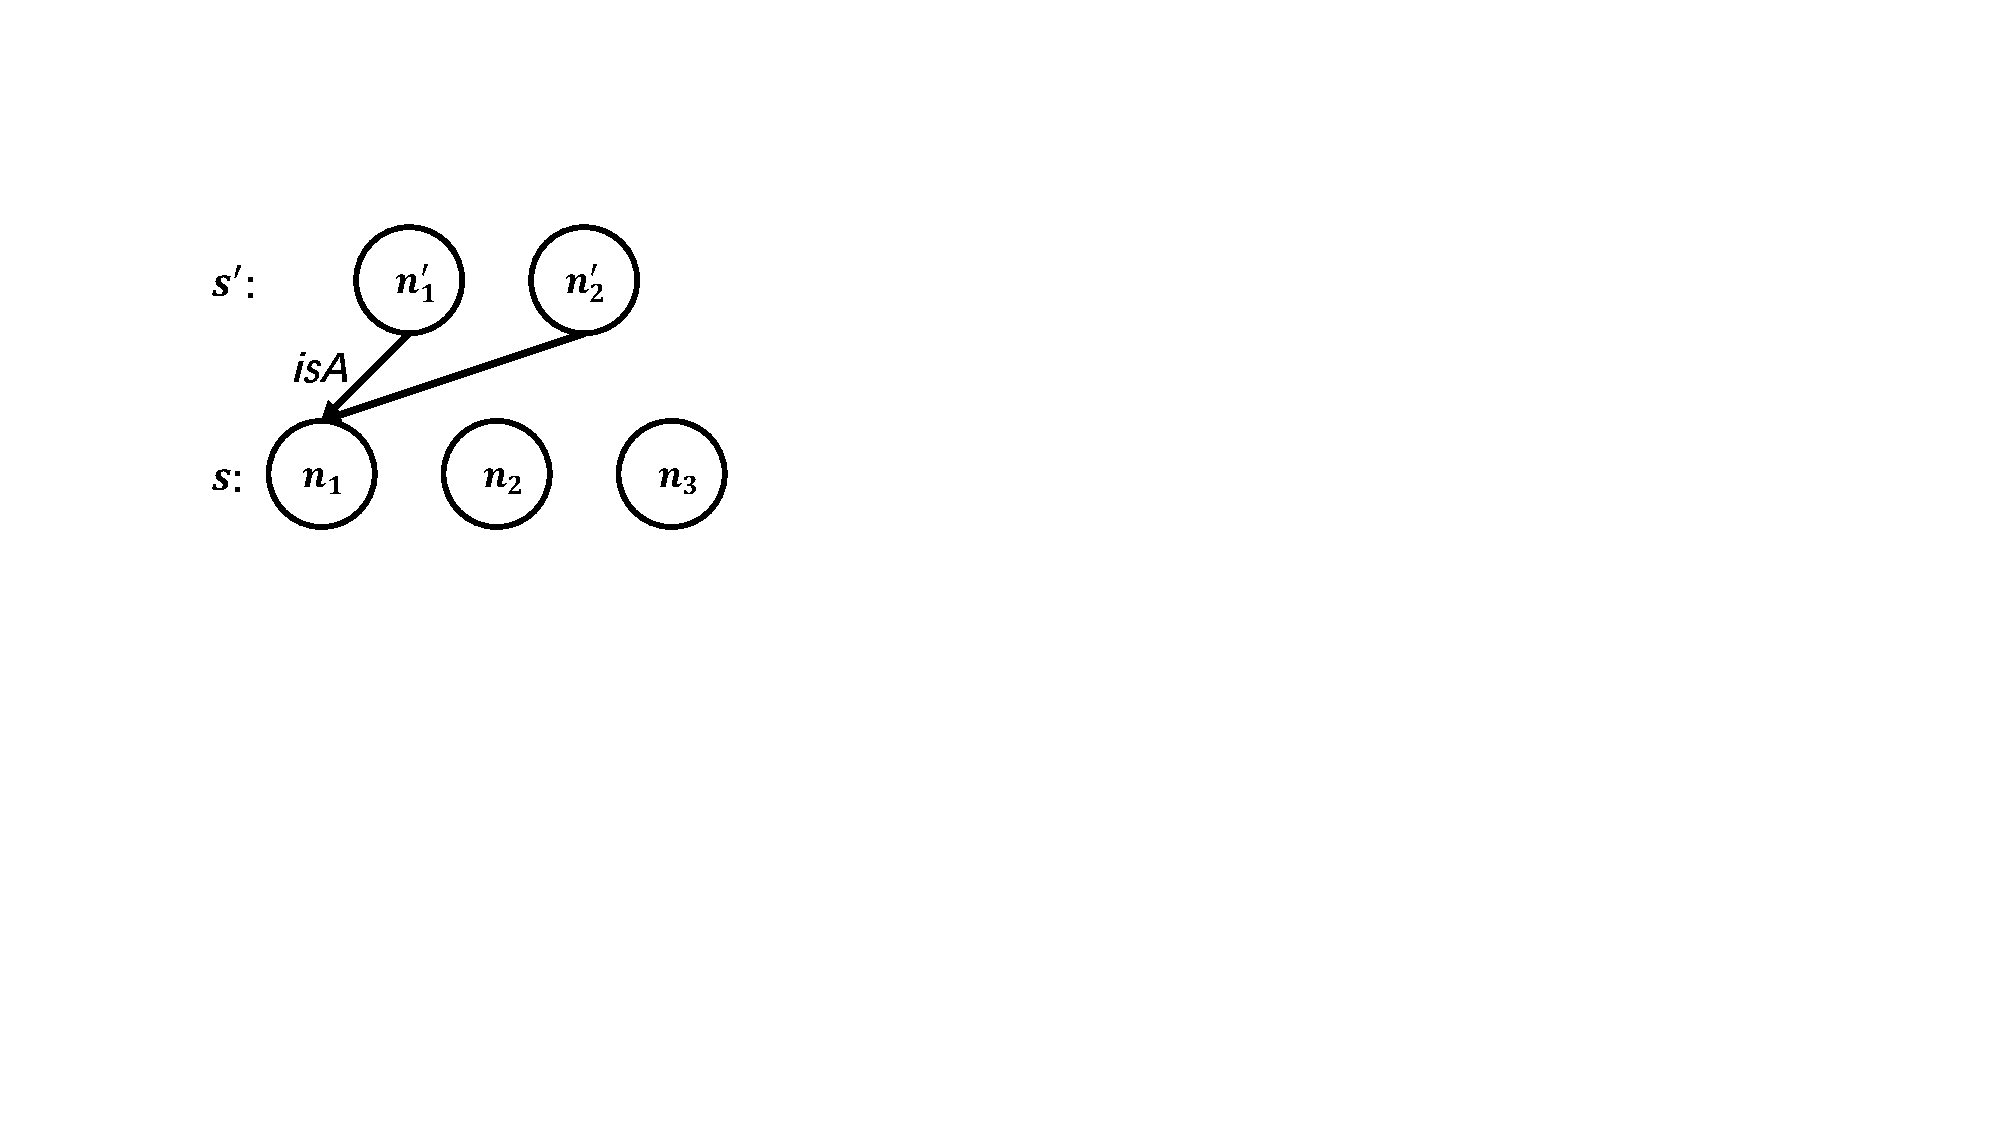
\includegraphics[width=.8\linewidth]{figures/subsumption_a}
		\caption{}
		\label{fig:subsumption_a}
	\end{subfigure}%
	\begin{subfigure}{.5\textwidth}
		\centering
		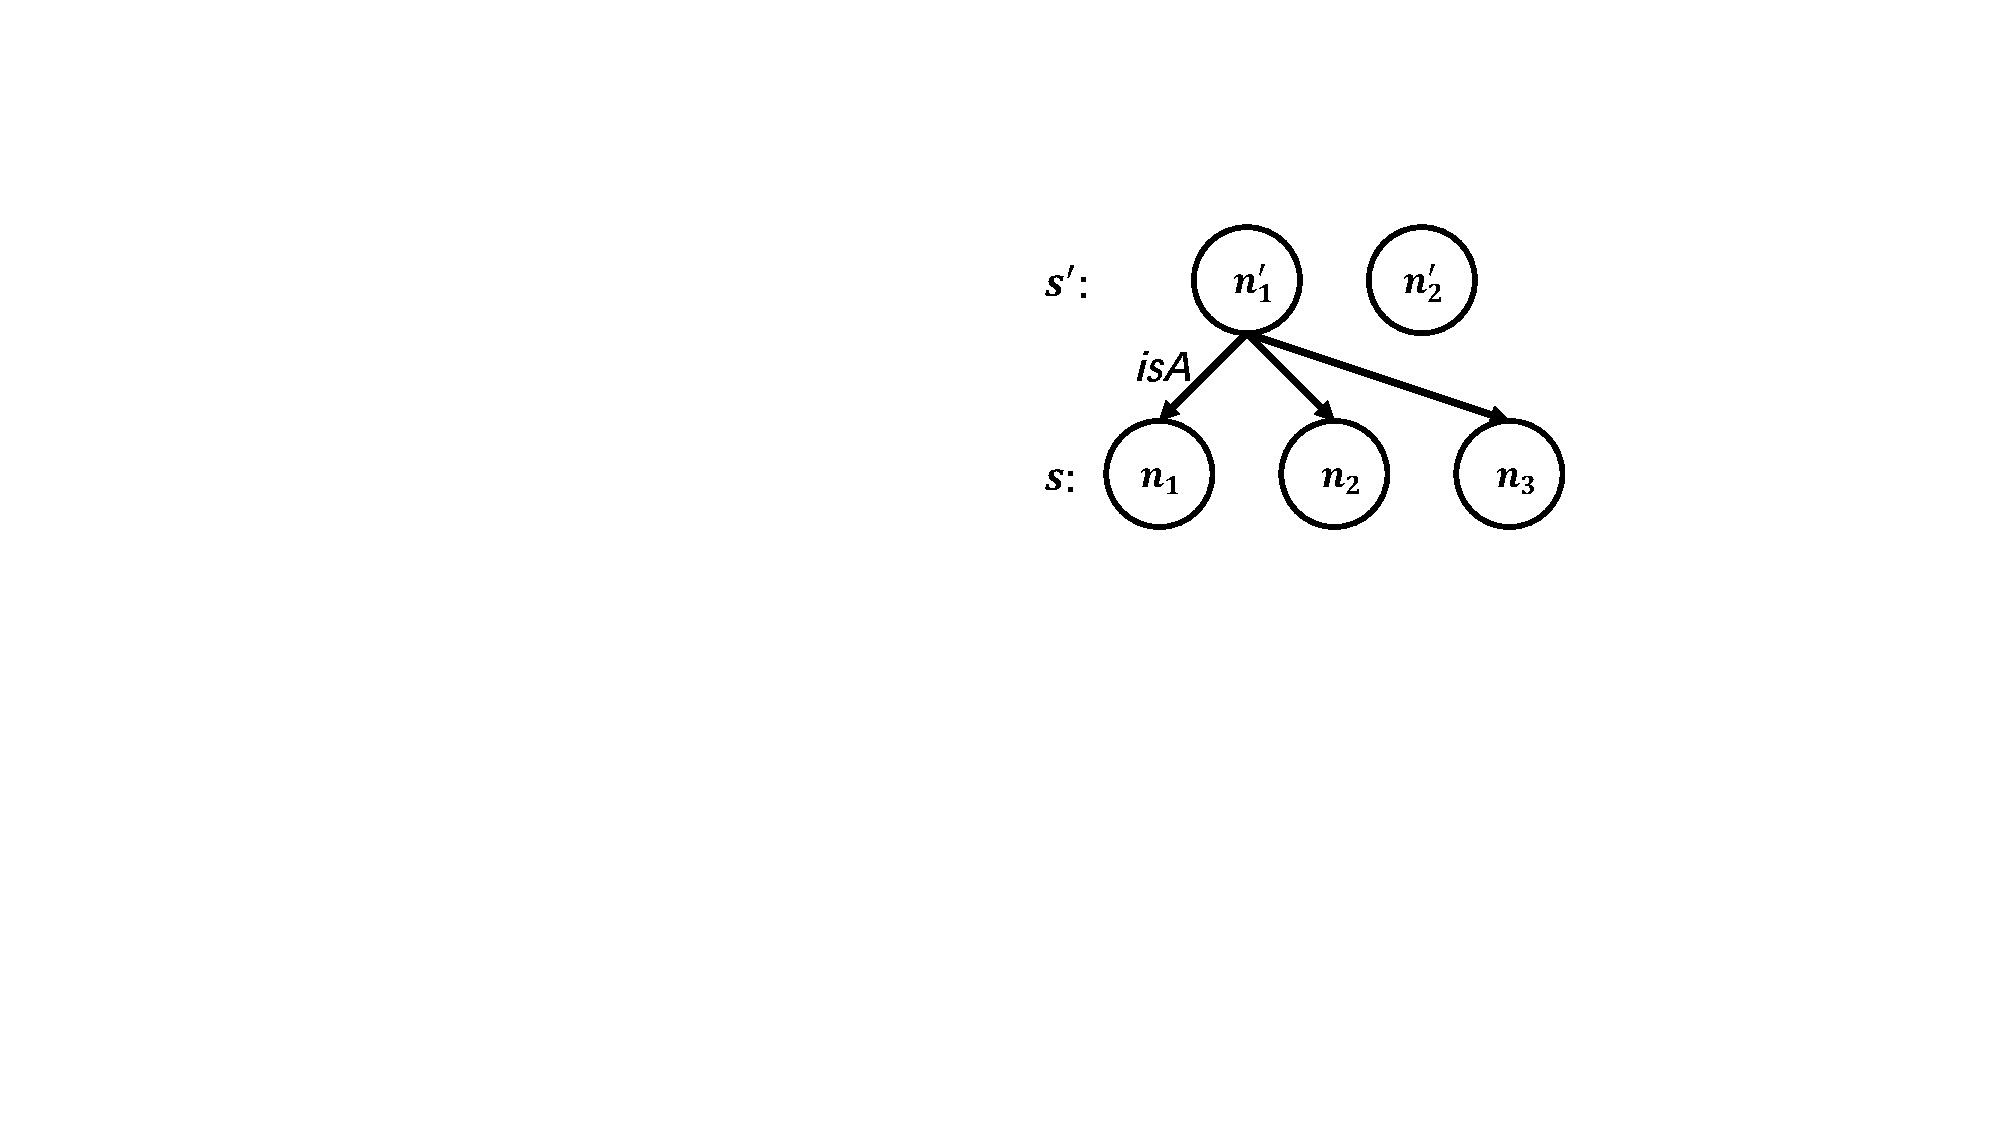
\includegraphics[width=.8\linewidth]{figures/subsumption_b}
		\caption{}
		\label{fig:subsumption_b}
	\end{subfigure}
	\caption{Two structures that $s'$ covers $s$}
	\label{fig:subsumption}
\end{figure}

Next, we group the aspect synsets $S=[s_1, s_2, ..., s_T]$
into aspect clusters $C=[c_1, c_2, ..., c_Q]$.
The intuition is that if $s$ is semantically covered 
by $s'$, 
which means they support the same prominent aspect,
then we group $s$ and $s'$ together.
Here, $s$ (e.g. $s=\{n_1, n_2, n_3\}$) and 
$s'$ (e.g. $s'=\{n'_1, n'_2\}$)
are aspect synsets.
We assume that the two structures 
shown in \figref{fig:subsumption} imply
the semantical subsumption.
Formally, structure (a) represents that 
$\exists n \in s$ such that
$\left\langle n',n \right\rangle \in E$
for $ \{\forall n', n'\in s'\}$. 
Similarly, structure (b) represents that 
$\exists n' \in s'$ such that
$\left\langle n',n \right\rangle \in E$
for $ \{\forall n, n\in s\}$. 
Either semantic coverage structure 
in \figref{fig:subsumption} should be
satisfied when $s$ is covered by $s'$.

The key to the grouping algorithm
is to decide the grouping order for the aspect synsets.
For example, $s$ could be covered by multiple 
aspect synsets, such as $s'$ and $s''$, 
It is too aggressive to group 
$s$, $s'$ and $s''$ into one aspect cluster directly.
We measure the semantic coverage using the 
\textit{relation weighting} scheme proposed in the previous step.
Formally, the semantic coverage of $s$ for $s'$ is
computed as: 
\begin{equation}
	cov(\left\langle s',s\right\rangle)=\displaystyle\max_{\left\langle u,v\right\rangle \in edges(\left\langle s',s\right\rangle)} w(\left\langle u,v\right\rangle)
	\label{eq:coverage}
\end{equation}
$edges(\left\langle s',s\right\rangle)$ is the set of edges
which are involved in the structures shown in \figref{fig:subsumption}.
$w(\left\langle u,v\right\rangle)$ is calculated as \eqnref{eq:weighing}.
Then, we sort the pairs of aspect synsets (e.g. $\left\langle s',s\right\rangle$) 
to be grouped together by their coverages $cov(\left\langle s',s\right\rangle)$ in descending order.

To control the purity of aspect clusters,
we propose an iterative algorithm to group those pairs.
We show the grouping details in \algoref{alg:grouping}.
The \textit{grouping rate} parameter determines how many
pairs to be grouped in each iteration.
The output of each iteration is a list of aspect clusters
feeding into the next iteration as inputs.

\begin{algorithm}[!th]
	\small
	\KwIn{A list of aspect synsets $S=[s_1, s_2, ..., s_T]$.}
	\KwOut{A list of aspect clustsers $C_{out}=[co_1, co_2, ..., co_Q]$}
	\BlankLine
	Initialize $C_{in}=[ci_1, ci_2, ..., ci_T]$, where $ci_t = s_t$\;
	\While{{\bf true}}{
		$C_{out} \leftarrow C_{in}$\;
		$pairs \leftarrow toGroup(C_{in})$\;
		\If{$len(pairs)=0$}{\bf break\;}
		Sort $\left\langle s',s\right\rangle \in pairs$ by $cov(\left\langle s',s\right\rangle)$ (\eqnref{eq:coverage}) in descending order,
		such that $pairs=[\left\langle s'_1,s_1\right\rangle, ..., \left\langle s'_K,s_K\right\rangle]$\;
		$combined \leftarrow \emptyset$\;
		$C \leftarrow []$\;
		\For{$i \leftarrow 1$ \KwTo $grouping\_rate$}{
%			$l \leftarrow len(C_{out})$\;
			$s \leftarrow s'_i \cup s_i$\;
			$combined \leftarrow combined \cup \{s'\} \cup \{s\}$\;
			Append $s$ to $C$\;
		}
	\For{$s \in C_{in}$ {\bf and} $s \notin combined$}{
		Append $s$ to $C$\;
	}
		Sort $C$ by priority (\eqnref{eq:priority}) in descending order\;
		$C_{in} \leftarrow C$\;
%		$C_{out} \leftarrow C$\;
	}
	{\bf return} $C_{out}$\;
	\caption{Grouping aspect clusters\label{alg:grouping}}
\end{algorithm}

Given the list of aspect clusters $C$, 
$toGroup(C)$ gives the pairs of aspect clusters which
satisfy the structures in \figref{fig:subsumption}.
Note that we set the \textit{grouping rate} as 1 in our algorithm
in order to avoid aggressive grouping.
After such grouping, each output aspect cluster ($co_{i}$)
can be seen as a coarse-grained aspect cluster.
To properly adjust the granularity and purity of $co_{i}$ 
($co_{i} \in C_{out}$),
we further cluster the aspects in $co_i$.
We represent each aspect $n$ as a vector described
in \eqnref{eq:embedding}
and use the K-means clustering method 
to cluster them.
The number of clusters $Z$ is auto-tuned using
silhouette score \cite{rousseeuw1987silhouettes}
\footnote{We empirically set the default silhouette score as $0.13$ for $Z=1$.}.

For example, after clustering, 
the $co_i$ splits into $Z$ clusters represented as
$co_i^{(1)}$, $co_i^{(2)}$, ..., 
and $co_i^{(Z)}$.
We treat such aspect clusters $co_i^{(j)}$ as 
fine-grained aspect clusters.
Each $co_i^{(j)}$ is associated with two priorities.
One is $priority(co_i^{(j)})$,
and the other is $priority(co_i)$ 
which is the priority of its corresponding
coarse-grained aspect cluster $co_i$.
We use $priority(co_i)$ as the first key and 
$priority(co_i^{(j)})$ as the second key to
sort the fine-grained aspect clusters $co_i^{(j)}$ in descending order.
The prominent aspects we expected are implied in those top 
fine-grained aspect clusters.

\subsection{Prominent Aspects Generation}
Finally, we generate the $K$ prominent aspects from 
the top fine-grained aspect clusters $co_i^{(j)}$.
We sort the aspects in $co_i^{(j)}$ by priority in descending
order, representing as 
$[n^{(i,j)}_1$, $n^{(i,j)}_2$, ..., $n^{(i,j)}_R]$.
Thus, $n^{(i,j)}_1$ is the most popular aspect
with the highest frequency $freq(n^{(i,j)}_1)$.

Next, we generate prominent aspects
from $co_i^{(j)}$ on three different cases:
\textit{Top-down case}, \textit{Bottom-up case}
and \textit{Miscellaneous case}.
We demonstrate the first two cases in \figref{fig:cases}.


\begin{figure}[!h]
	\centering
	\begin{subfigure}{.5\textwidth}
		\centering
		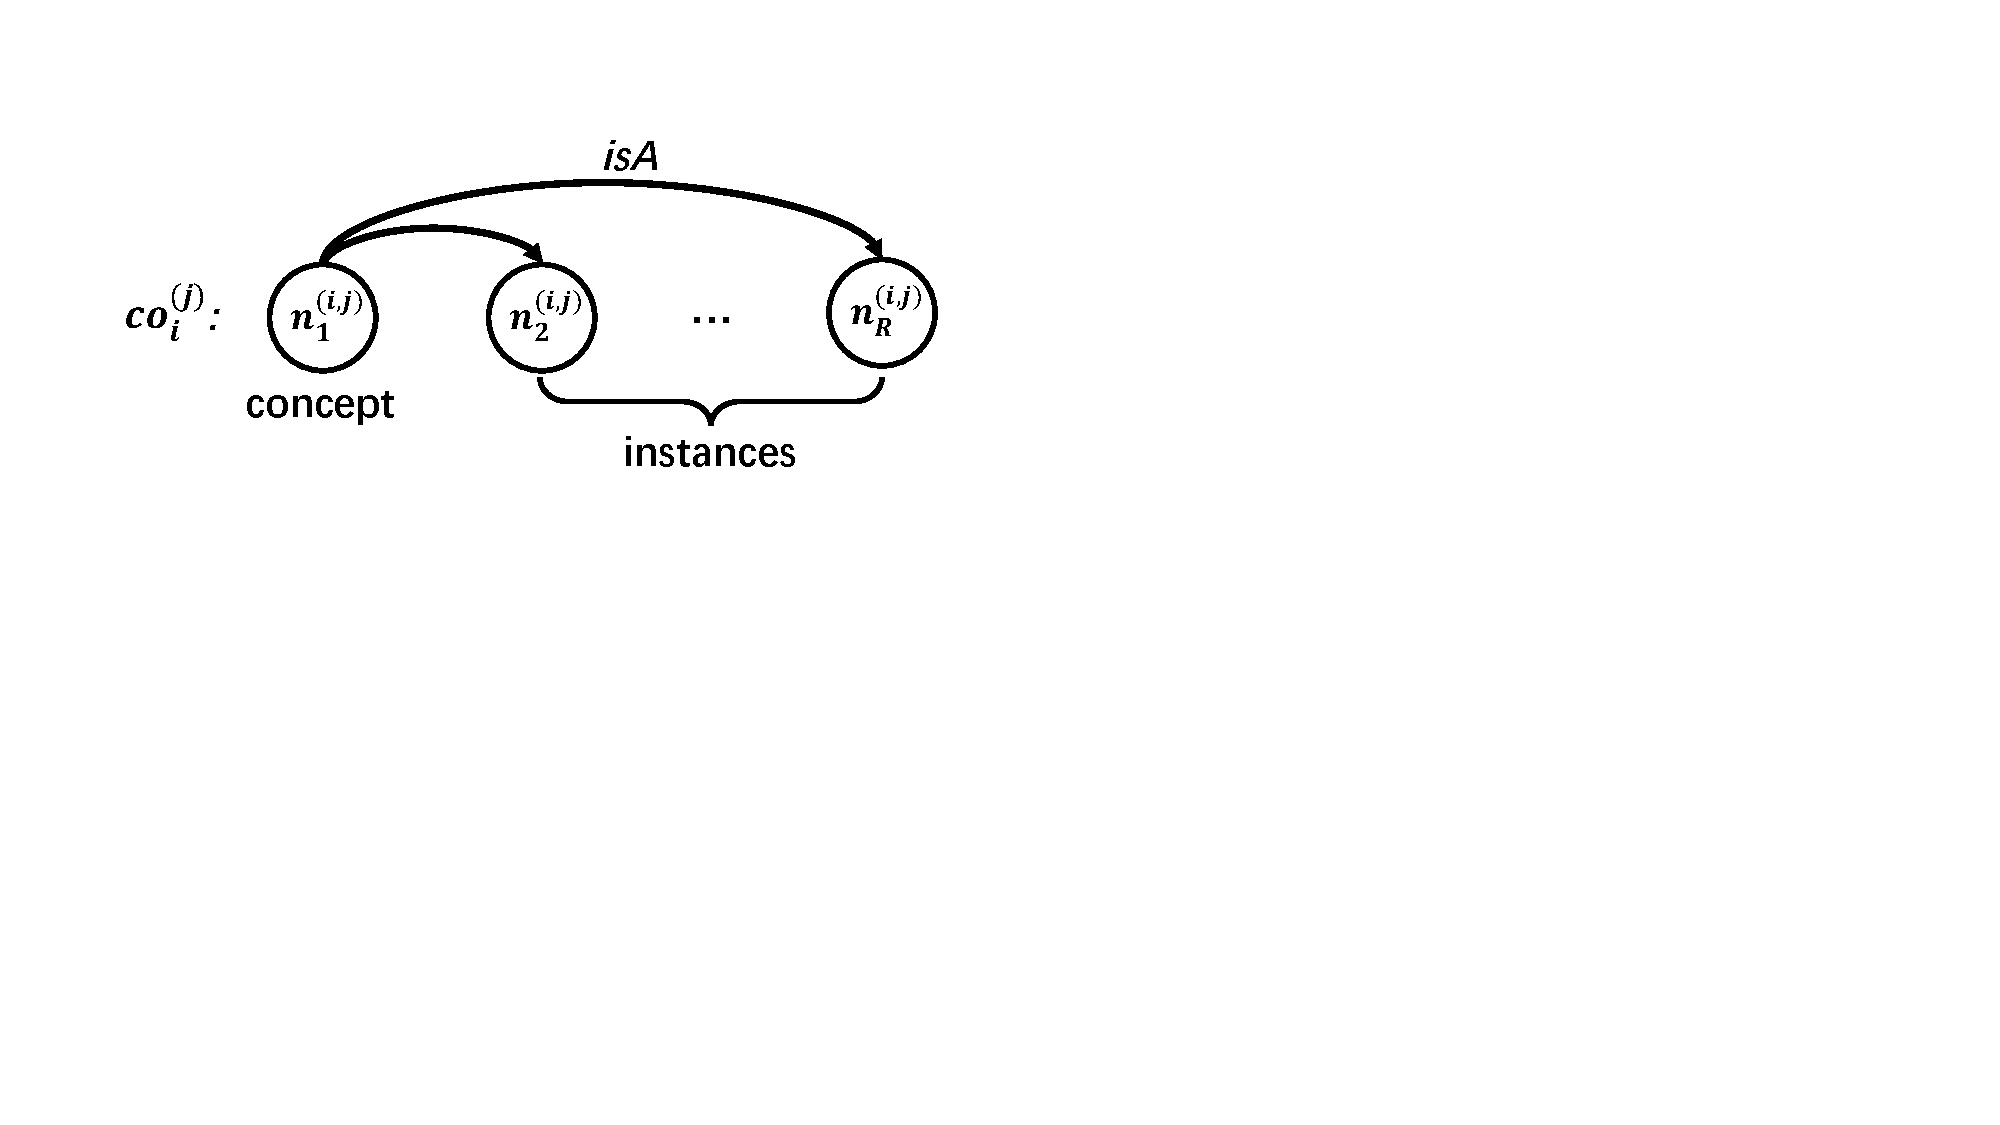
\includegraphics[width=0.95\linewidth]{figures/gaw}
		\caption{Top-down case}
		\label{fig:case_a}
	\end{subfigure}%
	\begin{subfigure}{.5\textwidth}
		\centering
		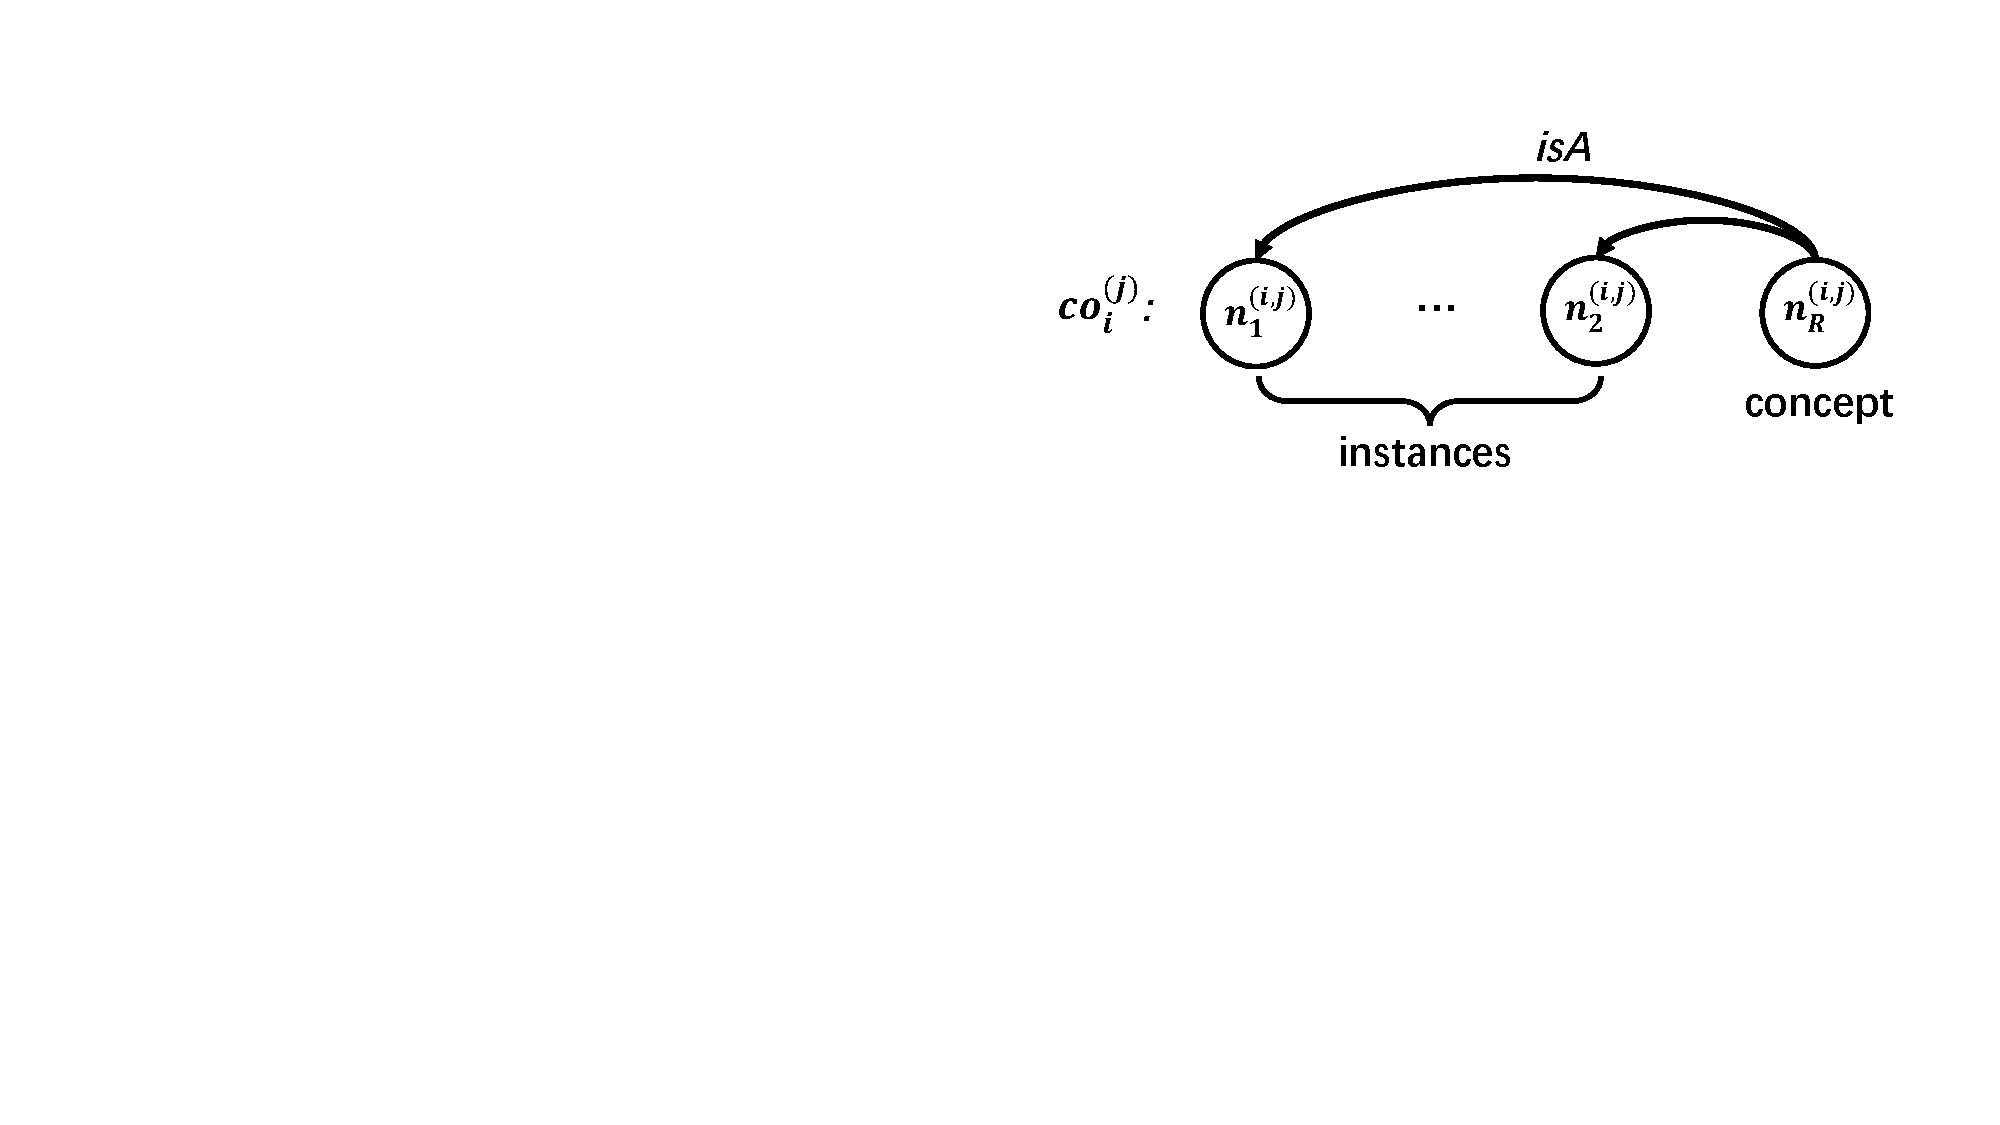
\includegraphics[width=0.95\linewidth]{figures/gbw}
		\caption{Bottom-up case}
		\label{fig:case_b}
	\end{subfigure}
	\caption{Different cases for prominent aspect generation from $co_i^{(j)}$}
	\label{fig:cases}
\end{figure}

\paragraph{Top-down case}
$n^{(i,j)}_1$ is the concept of $n^{(i,j)}_r ( 2 \le r \le R)$.
In other words, 
$n^{(i,j)}_r (2 \le r\le R)$ are the instances of $n^{(i,j)}_1$.
In this case, we extract the concept $n^{(i,j)}_1$ as the prominent aspect,
except that when $n^{(i,j)}_1$ is too vague (e.g. \textit{feature, service}), as well as
 $n^{(i,j)}_1$ do not dominate $co_i^{(j)}$,
then we extract the suboptimal aspect $n^{(i,j)}_2$ as the prominent aspect.
We formulate the domination constraint of  $n^{(i,j)}_1$ in $co_i^{(j)}$ as follows:
\begin{equation}
	\frac{freq(n^{(i,j)}_1)}{priority(co_i^{(j)})} \le \tau \footnote{$\tau = \frac{3}{4}$}
\end{equation}
Note that we measure the vagueness of each concept using Probase\cite{wu2012probase}.

\paragraph{Bottom-up case}
$n^{(i,j)}_R$ is the concept of $n^{(i,j)}_r ( 1 \le r \le R-1)$.
In this case, we extract the most popular instance $x$
and the concept $n^{(i,j)}_R$ as the prominent aspects.
Formally, 
\begin{equation}
x=\underset{n^{(i,j)}_r, 1 \le r \le R-1}{\operatorname{arg\,max}} f(n^{(i,j)}_r)
\end{equation}

\paragraph{Miscellaneous case}
All the other cases are divided as the miscellaneous case.
In this case, we simply extract the most popular aspect $n^{(i,j)}_1$ as the prominent aspect.

We perform above strategy along the sorted 
list of fine-grained aspect clusters
until we generate $K$ prominent aspects.
